\documentclass[a4paper,12pt]{article}
\usepackage{geometry}
\usepackage{indentfirst}
\usepackage{setspace}
\usepackage{amsmath}
\usepackage{amssymb}
\usepackage{graphicx}
\usepackage{wrapfig}
\usepackage{caption}
\usepackage{indentfirst}
\setlength{\parindent}{20pt}
\usepackage{amssymb}
\usepackage{float}
\usepackage{subcaption}

\graphicspath{ {./images/} }
\geometry{left=2.5cm, right=2.5cm, top=2.5cm, bottom=3cm}
\onehalfspacing

\begin{document}	
	\title{{\Huge Methods and Models for \\ Combinatorial Optimization} \\ Lab Exercise}
	\author{ Alexandre Rodrigues (2039952)}
	\date{\today}
	\maketitle
	
	
	\section*{Introduction}
		The objective of this exercise is to find the minimum time needed to drill all the holes in a electric panel.
		For part 1, I used the model described in the exercise text.
		For part 2, I used the Tabu Search with Aspiration Criteria, made some changes and added a heuristic initial solution procedure.
		
		\vspace{3cm}
		
		\begin{figure}[H]
			\centering
			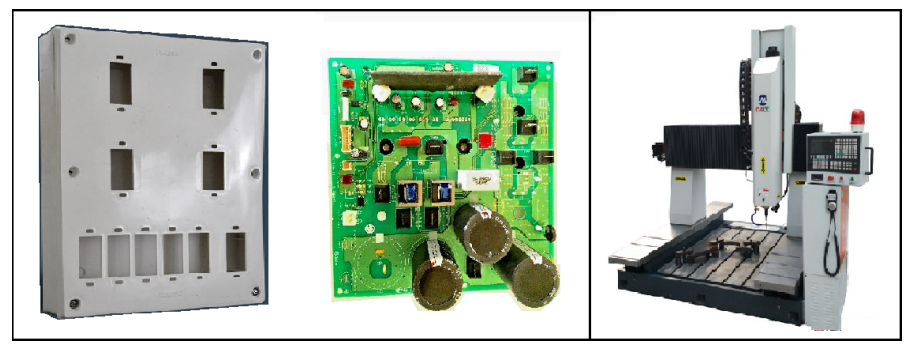
\includegraphics[width=.99\linewidth]{pic1.png}  
			\caption{Sample boards for electric panels and an automatic drilling machine}
			\label{fig:fig1}
		\end{figure}
	
	\pagebreak
	
	\tableofcontents
	
	\pagebreak
		
		
	\section{Technical Approach}
	
		\subsection{Mathematical formulation}
			This problem can be seen as a Traveling Salesmen Problem (TSP).
			We can represent it on a weighted complete graph $ G =(N,A) $, $ N $ being the set of nodes equivalent to the positions of the holes to be drilled, and $ A $ the arcs that correspond to the trajectory from one hole to another.
			The weight associated to each arc represents the time that the machine needs to move in that trajectory.
			The optimal solution is the minimum weight hamiltonian cycle on $ G $.
			
			A possible formulation is the follwing based on network flows.
			\begin{enumerate}
				\item Select a initial node (node 0);
				\item Set $ |N| - 1  $ as its outgoing flow;
				\item Push this flow towards the remaining nodes:
					\subitem $\diamond$ Each node is visited once;					
					\subitem $\diamond$ Each node receives 1 unit of flow;
					\subitem $\diamond$ Minimize the sum of $ c_{ij} $ over all the arcs that ship some flow.
			\end{enumerate}
			
			\hspace{-20pt}\textbf{Sets:}
			\begin{itemize}
				\item $ N = $ graph nodes, corresponding to the holes positions;
				\item $ A = arcs (i,j),\  \forall \ i,j \in N $, serving as the movement from hole $ i $ to hole $ j $.
			\end{itemize}
		
			\hspace{-20pt}\textbf{Parameters:}
			\begin{itemize}
				\item $ c_{ij} = $ time to move from $ i $ to $j,\forall (i,j) \in A $ ;
				\item $ 0 = $ arbitrary starting node, $ 0 \in N $.
			\end{itemize}
		
			\hspace{-20pt}\textbf{Decision variables:}
			\begin{itemize}
				\item $ x_{ij} = $ amount of the flow shipped from $ i $ to $j,\forall (i,j) \in A $ ;
				\item $ y_{ij} = 1 $ if arc $ (i,j) $ ships some flow, $ 0 $ otherwise, $\forall (i,j) \in A $ ;
			\end{itemize}
		
			The improved formulation in the exercise text is the following:
			\begin{align}
				min &\sum_{i,j:(i,j)\in A} c_{ij} y_{ij}\\
				s.t &\sum_{i:(i,k)\in A} x_{ik} - \sum_{j:(k,j),j\ne 0} x_{kj} 	&= 1 \qquad\qquad\qquad 	&\forall k \in N \backslash 0 \\
				&\sum_{j:(i,j)\in A} y_{ij}									   	&= 1 \qquad \qquad \qquad 	&\forall i \in N \\
				&\sum_{i:(i,j)\in A} y_{ij}									   	&= 1 \qquad \qquad \qquad 	&\forall j \in N \\
				&x_{ij}  													   	&\le (|N|-1) y_{ij} \quad 	&\forall (i,j) \in A, j\ne 0 \\
				&x_{ij}  \in R_+ 												&   						&\forall (i,j) \in A, j\ne 0 \\
				&y_{ij}  \in \{0,1\} 											&  							&\forall (i,j) \in A 
			\end{align}
		
		\subsection{Cplex Problem Setup}
			To solve this problem using the CPLEX callable API, we need to define all variables and constraints.
			The setup function receives the cost matrix as input.
			This matrix is computationally represented by a vector of vectors of doubles, so a vector of the rows of the matrix.
			To access an entry $ C_{ij} $ we use \texttt{C[i][j]}.
			
			The variables where saved in a similar fashion to the laboratory exercises with the following characteristics:
			\begin{enumerate}
				\item $x_{ij}$ ($ j \ne 0 $): integer, lower bound as $ 0 $, upper bound as $ +\infty $, not part of the objective function.
				\item $y_{ij}$ : binary ($ 0$ or $1$), with coefficient of the objective function as the entry of the cost matrix $ C_{ij} $	
			\end{enumerate}
			
			After the variables are saved in the problem, the indices will be:
			\begin{enumerate}
				\item $x_{ij}$ : \texttt{i*(N-1) + j-1}
				\item $y_{ij}$ : \texttt{N*(N+i-1) + j}
			\end{enumerate}
			
			The constraints $ \sum_{i:(i,j)\in A} y_{ij} = 1,\ \forall i \in N  $	and $ \sum_{j:(i,j)\in A} y_{ij} = 1,\ \forall j \in N  $ are identical except for the index we are iterating in.
			Implementation wise we can simply change the indices in the nested for loops.
			The coefficients of the variables will be all ones, the sense is \texttt{'E'} as equal and the right hand side is $ 1 $.
			
			The next constraint $ x_{ij} \le (|N|-1) y_{ij},\ \forall (i,j) \in A, j\ne 0 $ needs some rearranging.
			\begin{align}
				&x_{ij} 				 &\le &(|N|-1) y_{ij} \\
				&x_{ij} - (|N|-1) y_{ij} &\le &0\\	
				&x_{ij} + (1-|N|) y_{ij} &\le &0
			\end{align}
			Using this equivalent constraint we can set the variable coefficients as $ 1 $ and $ 1-|N| $ for x and y respectively.
			The sense will be \texttt{'L'} as less or equal and \texttt{rhs} $ 0 $.
			
			From the constraint $ \sum_{i:(i,k)\in A} x_{ik} - \sum_{j:(k,j),j\ne 0} x_{kj} = 1, \ \forall k \in N \backslash 0 $,	we can see that $x_{kk}$ appears twice with opposite signal.
			This allows us to get the following equivalent constraint:
			\begin{equation}
				\sum_{i:(i,k)\in A,i\ne k} x_{ik} - \sum_{j:(k,j),j\ne 0, j \ne k} x_{kj} = 1,  \quad \forall k \in N \backslash 0
			\end{equation}
			The number of variables in the original constraint is $2|N|-1 $, so now it is $ 2|N|-3 $.
			This approach was used to guarantee no errors when using the same variable index with different coefficient.
			We can set the variables coefficients as $ 1 $ in the first for loop and $ -1 $ in the second.
			The sense is \texttt{'E'} as equal and the \texttt{rhs} is $ 1 $.
			
			After this setup of the problem we can use the CPLEX API to solve it.
			
		\subsection{Additional Procedures}		 
			To simplify, reduce repetition and improve readability of the code, the following functions were created.
			
			\subsubsection{\texttt{readDists()}}
			\hspace{-20pt}\texttt{int readDists(const char* filename, std::vector<std::vector<double>>\& cost)}
					
				Similar to \texttt{read()} in the laboratory exercises. 
				Reads a file containing the number of nodes $ n $ in the first line and the cost matrix in the $ n $ following rows.
				Used in both parts of the work but for part 2 it calls the \texttt{setInfinite()} function to set its value as $ 2 \sum_{i,j} C_{ij}  $.
			
			\subsubsection{\texttt{readPos()}}
			\hspace{-20pt}\texttt{int readPos(const char* filename, std::vector<std::vector<double>>\& pos, \\ std::vector<std::vector<double>>\& cost)}
					
				Instead of the cost matrix it reads the nodes positions.
				Uses a file also with the number of nodes $ |N| $ in the first line and the positions in the $ |N| $ following rows.
				Saves them to a vector of $ |N| $ vectors of size $ 2 $, so $ (x_i, y_i) $ is equivalent to \texttt{(pos[i][0], pos[i][1])}.
				Calls \texttt{computeCost(n,pos,cost)} in the end.
				
			\subsubsection{\texttt{comupteCost()}}
				\hspace{-20pt}\texttt{void computeCost(const int n, const std::vector<std::vector<double>>\& pos, \\ std::vector<std::vector<double>>\& cost)}
					
				From the positions of the nodes it calculates the distances between each other.
				Uses 2 for loops and computes each entry of the cost matrix as the Manhattan distance of the two nodes:
					$$ Dist = |x_i-x_j| + |y_i-y_j| $$
				In part 2 this function calls \texttt{setInfinite()} to set its value as $ 2 \sum_{i,j} C_{ij}  $.
					
			\subsubsection{\texttt{unsigned long superSeed()}}
				Used to get a better seed for the pseudo random methods used to get the initial random solution for TSAC and the random holes positions.
				Is based on the Robert Jenkins' 96-bit Mix Function that uses 3 large integers, results of the functions: \texttt{clock()}, \texttt{std::time(NULL)}, \texttt{getpid()}.
				
				It was added because we got identical initial solutions when running the TSAC method time after time, meaning the change in time was not enough to change the seed.
				This is better because the process ID (PID) changes each time so it should have always a different result even if run immediately after.
				
			\subsubsection{\texttt{randomCost()}}
				\hspace{-20pt}\texttt{void randomCost(const int n, std::vector<std::vector<double>>\& pos, \\ std::vector<std::vector<double>>\& cost, const int classe)}
				
				This function creates random cost matrices from the number of nodes $ |N| $ and the class of instances defined by the user.
				Uses a nested for loop to compute all positions available in the $ |N| \times |N|  $ map (class 1) or $ (|N|-2) \times (|N|-2)  $  map (class 2).
				Then randomly shuffles this vector of positions and selects the first $ |N| $ points.
				Theses points are saved in the \texttt{pos} vector and the \texttt{computeCost()} function is called.
				The result of this function is a new cost matrix based on these random positions.
			
			\subsubsection{\texttt{PRINT\_ALL\_TPSOLVER}}
				This is a preprocessor variable used to enable or disable prints in the terminal, both for debug and to check the method's evolution.
				By default defined as $ 0 $ in line 147 (after \texttt{setupLP()}) of the \texttt{main.cpp} file in part 1 and in the top of \texttt{TSP.h} for part 2 (included in all files that use it).
				
		\subsection{Final Usability}
			\subsubsection{Part 1}
				The \texttt{main.cpp} file can be compiled using the given Makefile.
				Its usage is \texttt{./main filename.dat savedistsfile.dat [readDists] [Nrandom] [class]}.
				The first 2 arguments are mandatory. 
				The first is the file that will be read for information.
				The second is the file used to save the cost matrix: used to save the 30 instances that we tested with.
				\texttt{readDists} can be anything, if it is given, and there are no more arguments after, we read the file as the cost matrix instead of reading positions.
				\texttt{Nrandom} indicates the program to create a new random instance of size \texttt{Nrandom}.
				\texttt{class} is the class of instance we want to create, anything different from 1 indicates class 2, default is class 1.
				
				\textbf{Examples:}
				\begin{itemize}
					\item New random instance of class 2:\texttt{./main x New\_n10\_class2.dat x 10 2}
					\item Read from saved cost matrix:\texttt{./main SavedDists/n10\_class1/0.dat temp.dat x}
					\item Read from saved positions:\texttt{./main pos10/dists10\_1.dat SavedDists/dists10/1.dat}
				\end{itemize}
				Where \texttt{x} are disregarded, so it can be any letter, number or word.
							
			\subsubsection{Part 2}
				All needed files are compiled by the given Makefile.
				The program's usage is \texttt{./main filename.dat tabulength maxiter [init] [readPos] [Nrandom] [class]}
				The first 3 arguments are mandatory. 
				The first is the file that will be read for information.
				The other 2 arguments indicate the length of the tabu list and the maximum number of iterations respectively.
				\texttt{init} is 0 for random initial solution and 1 for the heuristic one, the default is random.
				\texttt{readPos} indicates the program that the file consists of the hole positions, if not given it will read the file as being the cost matrix.
				\texttt{Nrandom} indicates the program to create a new random instance of size \texttt{Nrandom}.
				\texttt{class} is the class of instance we want to create, different from 1 indicates class 2, default is class 1.
				
				\textbf{Examples:}
				\begin{itemize}
					\item New random instance of class 2:\texttt{./main x 6 20 1 x 10 2}
					\item Read from saved cost matrix:\texttt{./main SavedDists/n10\_class1/0.dat 6 10}
					\item Read from saved positions:\texttt{./main pos10/dists10\_1.dat 6 10 2 1}
				\end{itemize}
				Where \texttt{x} are disregarded, so it can be any letter, number or word.
					
		
		\subsection{Instancing}
			To fully understand this method we can use 3 classes of instances.
			
			\subsubsection{Class 1 - Random}
				Randomly selected $ |N| $ positions of the $ |N| \times |N| $ map and compute the cost matrix.
				
				\textbf{Implementation}:
				\begin{enumerate}
					\item Compute all possible positions ($ 3\times3 $ example)
					
					\begin{tabular}{|c|c|c|}
						\hline
						(0,0) & (0,1) & (0,2)  \\ \hline
						(1,0) & (1,1) & (1,2) \\ \hline
						(2,0) & (2,1) & (2,2) \\ \hline
					\end{tabular}
					\item Randomly shuffle them;
					\item Select the first $ |N| $ positions from the set.
				\end{enumerate}
				
			
			\subsubsection{Class 2 - Domain Specific Random}
				Same as before but for a $ (|N|-2) \times (|N|-2)  $ map.
				Each index is limited to \{$ 1 $, $ 2 $, $\ldots$ , $ |N|-2 $ \} instead of \{$ 0 $, $ 2 $, $\ldots$, $ |N|-1 $\}.
				This because there are basically no electric panels with holes near the border.
				
			\subsubsection{Class 3 - Handmade instances}
				For $ |N| = 10 $, I created the following 6 instances from what seemed more realistic.
				The first is an interpretation of the first image of figure \ref{fig:fig1}.
				I then created the positions files (folder \texttt{pos10}).
				
				\begin{figure}[H]
					\centering
					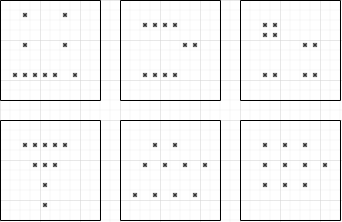
\includegraphics[width=.7\linewidth]{class3.png}  
					\caption{Instances of class 3}
					\label{fig:figsClass3}
				\end{figure}
			
					
			
		\subsection{Part 2}

			I started from the TSAC implementation from the Laboratory and added all the additional procedures to: randomly select holes positions, compute the costs matrix from these positions, read from positions files, better seed the random methods with a mix() function.
			
			As an additional study object, I made an heuristic initial solution computation based on the Nearest Neighbour.
			This can be done by iterating over the cost matrix and find the minimum value in each row, excluding the already visited nodes.
			Add this node to the cycle and continue on its row of the cost matrix.
			Hereby constructing a cycle that will be the initial solution.
			
			After some tests, I noticed that, in some cases, the method would return a worst solution that the initial.
			To solve this, I added a verification: if the best value at the end of the method is equal to the initial value, use the initial solution as the best one.
			
						
	
	\section{Results}
		I run 5 times the 6 handmade instances in class 3. 
		
		Both class 1 and 2 were tested using 30 random instances for $ 10 \le |N| \le 70 $.
		Due to the considerable time needed, 10 instances were tested for $ 80 \le |N| \le 100 $.
		Each instance was run 5 times to get the average computational time.
		
		The time to drill a hole is constant so we can disregard it.
		The total cost would be $ cost_{real}  = cost_{exp} + cN, c\in \mathbb{R}_+$.
		
		
		The following table resumes the results for class 3:
		\begin{table}[H]
			\centering
			\begin{tabular}{c|c|c|c}
				\textbf{Comparison}	& \textbf{exact} 	& \textbf{Random Initial}  		& \textbf{Heuristic Initial}  \\ \hline
				Time				& $ 0.1165 s $ 		& $ 4.05 \times 10^{-5} s $ 	& $ 1.06 \times 10^{-5} s $ \\ \hline
				Initial Value		& N/A		 		& $ 47.4 $ 						& $ 24.0 $ 					\\ \hline 
				Final Value			& $ 22.33 $	 		& $ 22.5 $ 						& $ 22.33 $ 				\\  
			\end{tabular}
			\caption{Comparison for class 3}
			\label{table:times3}
		\end{table}
	
		The TSAC method is clearly faster, an improvement of up to a factor of $ 10^4 $.
		Using an heuristic initial solution improves convergence time and final solutions found.
		One can also see that our initial heuristic solution is half of the random initial solution.
		This will be even more noticeable for larger $ |N| $, however the time differences (between the two TSAC scenarios) will become insignificant.
		
		The standard deviation of all values in table \ref{table:times3} never exceed 20\% of said value.
		
		
		As an initial objective we can see how fast the exact method was to solve class 1 and class 2 instances.
		\begin{table}[H]
			\centering
			\begin{tabular}{c|c|c}
				$\mathbf{|N|}$  & \textbf{Class 1} 	& \textbf{Class2}  \\ \hline
				$ 10  $			& $ 0.1199 s $ 		& $ 0.1285 s $ 		\\ \hline
				$ 20  $			& $ 0.430 s $ 		& $ 0.461 s $		\\ \hline
				$ 30  $			& $ 1.575 s $	 	& $ 1.397 s $ 		\\ \hline
				$ 40  $			& $ 6.603 s $ 		& $ 6.570 s $ 		\\ \hline
				$ 50  $			& $ 14.04 s $ 		& $ 14.55 s $ 		\\ \hline
				$ 60 $			& $ 28.80 s $ 		& $ 28.14 s $ 		\\ \hline
				$ 70 $			& $ 46.66s $	 	& $ 53.88 s $ 		\\ \hline
				$ 80 $			& $ 90.96 s $ 		& $ 86.53 s $ 		\\ \hline
				$ 90 $			& $ 215.1 s $	 	& $ 207.97 s $ 		\\ \hline
				$ 100 $			& $ 458.5 s $ 		& $ 312.64 s $ 		\\ 
			\end{tabular}
			\caption{Average Time for Exact}
			\label{table:times}
		\end{table}
		The fastest class to converge oscillates between each one when increasing $ |N| $, so we cannot conclude anything about that.		
				
		We can already answer the main question of part 1: assuming a max time as $ 20 $ seconds we can solve for up to $ 50 $ nodes.
		With 1 minute we go up to $ 70 $ nodes and the time increases somewhat exponentially afterwards.
		
		The largest standard deviations found was $ 105\% $ for $ |N| = 90$, $ 90\% $ for $ |N| = 100$ and $ 50\% $ for $ |N| = 30$.
		This large deviations can be due to other programs running on the server I used since these computations took so much time.
		
		
	\begin{table}[H]
		\centering
		\begin{tabular}{c|c|c|c|c}
			$ \mathbf{|N|}$ & \textbf{Class 1 RI}  & \textbf{Class1 HI}& \textbf{Class 2 RI} & \textbf{Class 2 HI}  \\ \hline
			$ 10  $			& $1.54\times10^{-5}$ & $9.35\times10^{-6}$& $1.97\times10^{-5}$ & $1.04\times10^{-5}$ \\ \hline
			$ 20  $			& $9.11\times10^{-5}$ & $1.40\times10^{-4}$& $1.00\times10^{-4}$ & $1.21\times10^{-4}$ \\ \hline
			$ 30  $			& $2.33\times10^{-4}$ & $2.54\times10^{-4}$& $2.31\times10^{-4}$ & $3.47\times10^{-4}$ \\ \hline
			$ 40  $			& $3.49\times10^{-4}$ & $7.53\times10^{-4}$& $3.42\times10^{-4}$ & $7.22\times10^{-4}$\\ \hline
			$ 50  $			& $7.97\times10^{-4}$ & $6.74\times10^{-4}$& $6.68\times10^{-4}$ & $9.80\times10^{-4}$ \\ \hline
			$ 60  $			& $1.13\times10^{-3}$ & $2.18\times10^{-3}$& $1.70\times10^{-3}$ & $2.05\times10^{-3}$ \\ \hline
			$ 70 $			& $1.91\times10^{-3}$ & $2.54\times10^{-3}$& $3.16\times10^{-3}$ & $3.11\times10^{-3}$\\ \hline
			$ 80 $			& $2.56\times10^{-3}$ & $3.96\times10^{-3}$& $2.97\times10^{-3}$ & $3.07\times10^{-3}$\\ \hline
			$ 90 $			& $4.98\times10^{-3}$ & $5.93\times10^{-3}$& $3.87\times10^{-3}$ & $5.73\times10^{-3}$\\ \hline
			$ 100 $			& $5.83\times10^{-3}$ & $8.20\times10^{-3}$& $5.14\times10^{-3}$ & $8.66\times10^{-3}$\\
		\end{tabular}
		\caption{Average Time for TSAC}
		\label{table:times2}
	\end{table}
	Note: RI - Random Initial Solution, HI - Heuristic Initial Solution.
	
	There were no significant differences between the classes and initialization methods used.
	All this computational times are below $ 1 $ second, so very easily solvable.
	As an extra test, for $ |N| = 1000 $, obtaining times of around $ 5 $ seconds.
	
	The largest standard deviations of computational time found were around $40\%$, being usually of $25\%$.
	
	The following tables show the final solution values obtained.

	\begin{table}[H]
		\centering
		\begin{tabular}{c|c|c|c|c|c}
			$ \mathbf{|N|}$	& \textbf{CPLEX}& \textbf{Initial RI}   & \textbf{Final RI}	& \textbf{Initial HI} 	& \textbf{Final RI} \\ \hline
			$ 10  $			& $ 34.067 $ 	& $ 66.067 $ 			& $ 34.067 $  		& $ 38.067 $ 			& $ 34.067 $		\\ \hline
			$ 20  $			& $ 94.33 $ 	& $ 258.2 $ 			& $ 95.067 $  		& $ 110.8 $ 			& $ 94.933 $		\\ \hline
			$ 30  $			& $ 167.067 $ 	& $ 606.53 $ 			& $ 170.2 $  		& $ 202.6 $ 			& $ 169.6 $ 		\\ \hline
			$ 40  $			& $ 257.4 $ 	& $ 1076.87 $ 			& $ 266.3 $  		& $ 310.8 $ 			& $ 263.93 $ 		\\ \hline
			$ 50  $			& $ 356.6 $ 	& $ 1630.47 $ 			& $ 366.8 $  		& $ 428.067 $ 			& $ 366.467 $ 		\\ \hline
			$ 60  $			& $ 461.93 $ 	& $ 2418.6 $ 			& $ 482.73 $  		& $ 570.4 $ 			& $ 479.267 $ 		\\ \hline
			$ 70 $			& $ 578.93 $ 	& $ 3264.13 $ 			& $ 607.93 $ 	 	& $ 732.73 $	 		& $ 599.6 $ 		\\ \hline
			$ 80 $			& $ 703.4 $ 	& $ 4343.2 $ 			& $ 739.6 $  		& $ 869.6 $ 			& $ 724.2 $ 		\\ \hline
			$ 90 $			& $ 833.6 $ 	& $ 5476.8 $ 			& $ 888.2 $  		& $ 1052.2 $ 			& $ 869 $ 			\\ \hline
			$ 100 $			& $ 976.6 $ 	& $ 6670.2 $ 			& $ 1042 $  		& $ 1228.2 $ 			& $ 1013.4 $ 		\\
		\end{tabular}
		\caption{Initial and Final Solutions for Class 1}
		\label{table:sols}
	\end{table}

	The largest standard deviations of initial solutions found were around $18\%$, being usually of $10\%$.
	For final solutions the largest ones were around $35\%$.
	Solutions using heuristic initial solutions are up to $4\%$ larger than the optimal, for RI it is up to an $6.5\%$ increment, for $|N| = 90,100$.
	The smallest differences are for smaller $ |N| $, where they are almost insignificant.
	
	\begin{table}[H]
		\centering
		\begin{tabular}{c|c|c|c|c|c}
			$ \mathbf{|N|}$	& \textbf{CPLEX}& \textbf{Initial RI}   & \textbf{Final RI}	& \textbf{Initial HI} 	& \textbf{Final RI} \\ \hline
			$ 10  $			& $ 28.533 $ 	& $ 52.333 $ 			& $ 28.533 $  		& $ 32 $ 				& $ 28.533 $		\\ \hline
			$ 20  $			& $ 84.467 $ 	& $ 233.13 $ 			& $ 84.733 $  		& $ 98 $ 				& $ 84.6$			\\ \hline
			$ 30  $			& $ 160.933 $ 	& $ 562.73 $ 			& $ 164.4 $  		& $ 197.53 $ 			& $ 163.067 $ 		\\ \hline
			$ 40  $			& $ 243.4 $ 	& $ 1040.4 $ 			& $ 252.53 $  		& $ 289.33 $ 			& $ 248.8 $ 		\\ \hline
			$ 50  $			& $ 339.73 $ 	& $ 1583.53 $ 			& $ 350.2 $		  	& $ 412.4 $ 			& $ 346.53 $ 		\\ \hline
			$ 60  $			& $ 445 $ 		& $ 2356.67 $ 			& $ 466.2 $  		& $ 527.93 $ 			& $ 458.267 $	 	\\ \hline
			$ 70 $			& $ 560.13 $ 	& $ 3203.8 $ 			& $ 593.6 $  		& $ 898.867 $ 			& $ 582.4 $ 		\\ \hline
			$ 80 $			& $ 687.6 $ 	& $ 4163.4 $ 			& $ 730 $  			& $ 859.8 $ 			& $ 711.2 $ 		\\ \hline
			$ 90 $			& $ 815.4 $ 	& $ 5358.4 $ 			& $ 845.4 $  		& $ 1016 $ 				& $ 845 $ 			\\ \hline
			$ 100 $			& $ 951.8 $ 	& $ 6665 $ 				& $ 1022 $  		& $ 1172.2 $ 			& $ 988$ 			\\
		\end{tabular}
		\caption{Initial and Final Solutions for Class 2}
		\label{table:sols2}
	\end{table}
	For class 2,  the largest standard deviations of initial solutions found were around $17\%$, being usually of $10\%$.
	For final solutions the largest ones were around $11\%$.
	
	Solutions using heuristic initial solutions are up to $4\%$ larger than the optimal, for RI it is up to an $6\%$ increment, for $|N| = 70$.
	The smallest differences are for smaller $ |N| $, where they are almost insignificant.

	Class 2 has smaller objective function values as expected.
	
	\section{Conclusions}
	
		The TSAC method is very fast and can get almost optimal solutions for small $ |N| $.
		For large $ |N| $ the CPLEX method is very slow but can be the better option if we want to reduce the drilling time as much as possible.
		In this case, the best approach seems to use an heuristic initial solution and TSAC, when we want fast but good results.
		
		When using the heuristic initial solution we get a better approximation to the optimal solution.
		Although theoretically there is no guarantee that starting from a better solution gets us a better final solution, this was mostly the case for this implementation.
		We can although notice a tendency to worse solutions when we increase $ |N| $.
		
		When the goal is to minimize drilling time on an board with more the 50 holes, a company would benefit to take some time to compute the best machine paths and thus get an up to $5\%$ time saving in all pieces drilled.
		If the company wants to drill a small quantity of boards or boards with little holes, the TSAC method with heuristic initial solution is the best.
	
	
\end{document}



